%! Author = Dean
%! Date = 12/30/2023

\chapter{Treniranje i optimizacija}\label{ch:treniranje-i-optimizacija}

Kao što smo vidjeli ranije, konvolucijske neuronske mreže imaju ogromnu količinu parametara, a da bi naš model bio što točniji moramo mu postaviti ispravne parametre a to postižemo treniranjem.
Da bi mogli uopće trenirati mrežu, trebaju nam podatci nad kojim ćemo ga trenirati.
Kako ne bi pretrenirali model, podatke dijelimo na testne podatke i podatke za ispitivanje u omjeru 70% za treniranje i 30% za testiranje.
Svrha podjele je istrenirati mrežu nad testnim podatcima, a zatim, na temelju rezultata nad podatcima za ispitivanje, podesiti hiperparametre ako je potrebno kako bi se poboljšala generalizacija modela.
Proces treniranja koristi propagaciju greške unatrag, koji smo obradili ranije.

Imamo razne načine optimiranja, ali ovdje ću obraditi najjednostavniji - gradijentni spust.
Ideja iza gradijentnog spusta je pronaći minimum funkcije gubitka iterativnim izračunavanjem gradijenta i kretanjem prema njemu.
Problem kod ovog načina je ako funkcija gubitka nije konveksna, odnosno ako ima lokalnih minimuma, gdje gradijentni spust može zapeti.
Osim toga, nemamo određenu početnu točku već ju nasumično biramo, pa vrijeme i točnost modela ovise o početnoj točki.

\FloatBarrier
\begin{figure}[h]
    \centering
    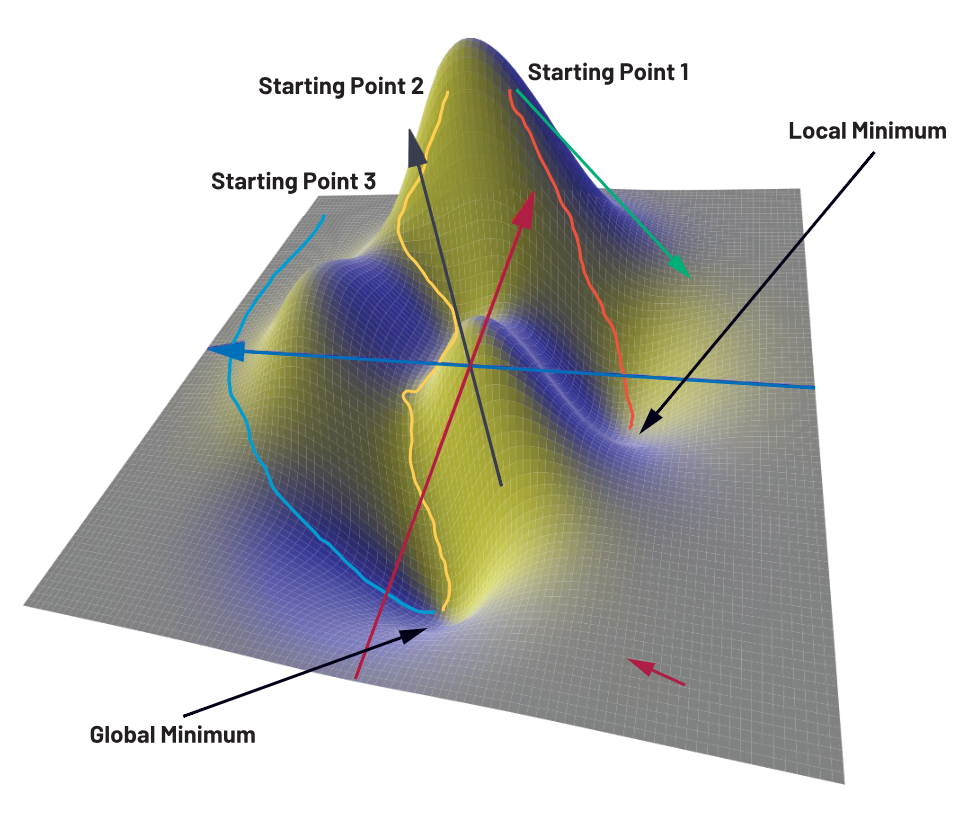
\includegraphics[width=0.8\textwidth]{images/Gradijentni-spust}
    \caption{Gradijentni spust}
    \label{fig:slika18}
\end{figure}
\FloatBarrier

Često do loše generalizacije dolazi zato što nam je model presložen, što znači da se lako prilagodi šumovima koji se nalaze u testnim podatcima.
Zato se u optimizaciju uvodi regularizacija.
Regularizacija nam omogućava da krenemo od vrlo složenog modela i onda će nam sama regularizacija tijekom treniranja smanjivati složenost modela.
L2 i L1 regularizacija je popularna i ona se direktno može ubaciti u funkciju gubitka, ali puno češće se koristi tehnika koju smo već objasnili a to je \emph{dropout}.
Važno je napomenuti da treba biti oprezan pri odabiru jačine regularizacije, jer ako je prejaka regularizacija model će biti prejednostavan, podnaučen model, te će isto loše generalizirati.
Isto tako slaba regularizacija neće uopće utjecat na složenost modela te će se model opet prilagodit šumovima i dobit ćemo prenaučen model.
Tako da za dropout metodu treba pažljivo odabrati hiperparametar p koji govori koliko će neurona \enquote{ugasiti} tijekom jedne iteracije treniranja.